\documentclass[10pt, xcolor={dvipsnames}]{beamer}

\usepackage{minted}
\usepackage{subfiles}
\usepackage{amsmath,amssymb,amsthm,commath,mathtools}
\usepackage{esint}
\usepackage{enumerate}
\usepackage{subcaption}
\usepackage{graphicx}
\usepackage{adjustbox}
\usepackage{soul}
\usepackage{booktabs}
\usepackage{tabularx}
\usepackage{environ}
\usepackage{etoolbox}
\usepackage{yfonts}
\usepackage[dutch]{babel}
\usepackage[utf8]{inputenc}
\usepackage{marvosym}
\usepackage[style=numeric]{biblatex}
\usepackage{textcomp}
\usepackage{hyperref}
\usepackage{xkeyval}
\usepackage[T1]{fontenc}
\usepackage{textgreek}
\usepackage{lmodern}
\usepackage[version=4]{mhchem}
\usepackage{ragged2e}
\usepackage{import}
\usepackage{multicol}
\usepackage{csquotes}
\usepackage{tcolorbox}
\usefonttheme[onlymath]{serif}
\newcommand{\error}{\textbf{\textcolor{red}{ERROR!}}}
\newcommand{\Norm}[1]{\left\lVert#1\right\rVert}
\usetheme{Dresden}
\setbeamertemplate{navigation symbols}{}

\title{\LaTeX{}-cursus Week 2}
\author{\TeX niCie}
\date{3 oktober 2022}

\DeclareMathOperator{\atantwee}{atan2}

\DeclareMathOperator{\beeld}{beeld}

\DeclareMathOperator{\kernel}{ker}


\newcommand{\abcformule}{\frac{-b \pm \sqrt{b^2-4ac}}{2a}}
\newcommand{\abcformuleX}[3]{\frac{-#2 \pm \sqrt{#2^2-4\cdot#1\cdot#3}}{2\cdot#1}}
\makeatletter
\newcommand{\currentfontsize}{\fontsize{\f@size}{\f@baselineskip}\selectfont}
\makeatother
% Als je het bestand dumpt naar een format, worden packages hierna niet meegedumpt maar elke keer
% fris ingeladen
\csname endofdump\endcsname
\usepackage{etoolbox}
\AtBeginEnvironment{tcolorbox}{\small}
\setminted[tex]{fontsize=\small, autogobble=true, linenos=true, frame=single}
\usepackage{tcolorbox}
\setmintedinline{fontsize=\currentfontsize}
\begin{document}

\begin{frame}
	\titlepage
	\centering

	Please log in (or create an account) on \url{overleaf.com}
\end{frame}
\begin{frame}[fragile]{LaTeX commands}
    LaTeX commando's beginnen met een backslash \textbackslash, gevolgd door letters of een speciaal teken: \@, \#, \%, \ldots.

    Commando's kunnen \textbf{argumenten} en \textbf{optionele argumenten} hebben.

    \begin{minted}[autogobble,numbers=none]{tex}
        \commando
    \end{minted}
    of
    \begin{minted}[autogobble,numbers=none]{tex}
        \commando{argument}
    \end{minted}
    of
    \begin{minted}[autogobble,numbers=none]{tex}
        \commando{argument1}{argument2}
    \end{minted}
    or
    \begin{minted}[autogobble,numbers=none]{tex}
        \commando[optioneel argument]{argument}
    \end{minted}

\end{frame}
\copyrightTim

\begin{frame}[fragile, t]{Simple document in \LaTeX}
	%autogobble removes extra tabs we want in the code but should not be in the pdf code display
	\begin{columns}
        \begin{column}{0.3\textwidth}
	\begin{minted}[autogobble, linenos=true, escapeinside=||]{tex} 
	\documentclass{article}


	\begin{document}
	



	\end{document}
	\end{minted}
\end{column}
\begin{column}{0.1\textwidth}
	{\Huge \textcolor{red}{ \} } }\\[1.5cm]
	{\Huge \textcolor{red}{ \} } }
\end{column}
\begin{column}{0.5\textwidth}
	\textbf{preamble}: document settings go here\\[1.5cm]
	\textbf{body}: content (text and images) goes here\\[2cm]
\end{column}
\end{columns}

\end{frame}
\copyrightTim

\begin{frame}[fragile, t]{Simple document in \LaTeX}
	%autogobble removes extra tabs we want in the code but should not be in the pdf code display
	\begin{columns}
        \begin{column}{0.5\textwidth}
	\begin{minted}[autogobble, linenos=true, escapeinside=||]{tex} 
	\documentclass{article}

		
	\begin{document}

	The Differential and Integral 
	Calculus, or, as it was formerly 
	called in this country, 
	the Doctrine of Fluxions, has always 
	been supposed to present remarkable 
	obstacles to the beginner.

	\end{document}
	\end{minted}

	Example text: \"Elementary Illustrations of the Differential and Integral Calculus\" by Augustus De Morgan
\end{column}
\begin{column}{0.05\textwidth}
	\phantom{{\Huge \textcolor{red}{ \} } }}
	\\[2cm]
	{\Huge \textcolor{red}{ \} } }
	
\end{column}
\begin{column}{0.4\textwidth}
	\phantom{\textbf{preamble}: document settings go here}
	\\[2cm]
	\textbf{body}: content (text and images) goes here
\end{column}
\end{columns}

\end{frame}

\copyrightTim

\begin{frame}[fragile, t]{Een eenvoudig document in \LaTeX}
	%autogobble removes extra tabs we want in the code but should not be in the pdf code display
	\begin{columns}[t]
        \begin{column}{0.5\textwidth}
			\vspace{-20pt}
	\begin{minted}[autogobble, linenos=true, escapeinside=||]{tex} 
	\documentclass[a4paper,11pt]{article}

		
	\begin{document}

	The Differential and Integral 
	Calculus, or, as it was formerly 
	called in this country, 
	the Doctrine of Fluxions, has always 
	been supposed to present remarkable 
	obstacles to the beginner.

	\end{document}
	\end{minted}

	{\tiny
	Example text: ``Elementary Illustrations of the Differential and Integral Calculus''
	by Augustus De Morgan
	\par}
\end{column}
\begin{column}{0.05\textwidth}
	\vspace{0pt}

	{\Huge \textcolor{red}{ \} } }
	\\[1.5cm]
	\phantom{{\Huge \textcolor{red}{ \} } }}
	
\end{column}
\begin{column}{0.4\textwidth}
	\vspace{0pt}
	
	\textbf{preamble}: instellingen hier
	\\[1.5cm]
	\phantom{\textbf{body}: inhoud (tekst, plaatjes, tabellen) hier}
\end{column}
\end{columns}

\end{frame}

\begin{frame}[fragile]{tekst uitlijnen}
    
    \begin{flushright}
            rechts uitgelijnd
    \end{flushright}

    \begin{flushleft}
        links uitgelijnd
    \end{flushleft}

    \begin{center}
        gecentreerd
    \end{center}

    \begin{minted}[highlightlines={1,5,9}]{tex}
    \begin{flushright}
        deze tekst staat rechts uitgelijnd
    \end{flushright}

    \begin{flushleft}
        deze tekst staat links uitgelijnd
    \end{flushleft}

    \begin{center}
        deze tekst staat gecentreerd
    \end{center}
    \end{minted}

\end{frame}
\begin{frame}[fragile]{Wiskundepackages}
De onderstaande drie packages zijn handig om wiskunde te zetten:
\begin{minted}[highlightlines={2,3,4}]{tex}
\documentclass[a4paper, 10pt]{article}
\usepackage{amsmath}
\usepackage{amssymb}
\usepackage{amsthm}
\begin{document}
\begin{align}
    ax^2 + bx + c &= 0 && 
    \text{kwadratische vergelijking} 
    ax^3 + bx^2 + cx + d &= 0 && 
    \text{derdegraadsvergelijking}
\end{align} 
\end{document}
\end{minted}

Met deze packages kun je tekst toevoegen aan formules, 
extra symbolen gebruiken zoals \( \boxplus \) , \( \leadsto \) en \(\mathbb{R}\) betere environments voor stellingen en bewijzen gebruiken.

\end{frame}
\begin{frame}[fragile]{Wiskundepackages}
De onderstaande drie packages zijn handig om wiskunde te zetten:
\begin{minted}[highlightlines={2,3,4}]{tex}
\documentclass[a4paper, 10pt]{article}
\usepackage{amsmath}
\usepackage{amssymb}
\usepackage{amsthm}
\begin{align}
    ax^2 + bx + c &= 0 && 
    \text{kwadratische vergelijking} \\
    ax^3 + bx^2 + cx + d &= 0 && 
    \text{derdegraadsvergelijking}
\end{align} 
\end{minted}
\begin{tcolorbox}[width=11cm,fontupper=\footnotesize, fontlower=\footnotesize]
\begin{align*}
    ax^2 + bx + c &= 0 && 
    \text{kwadratische vergelijking} \\
    ax^3 + bx^2 + cx + d &= 0 && 
    \text{Dderdegraadsvergelijking}
\end{align*} 
\end{tcolorbox}

\end{frame}
\copyrightTim

\begin{frame}[fragile]{Wiskunde}
Er zijn twee manieren om wiskunde te zetten:

\begin{tcolorbox}[width=13cm, title={inline mode}, size=small]
    The trigonometric identity is given by \( \sin^2(\theta) + \cos^2(\theta) = 1 \) for all \( \theta \).
\end{tcolorbox}

 \begin{tcolorbox}[width=13cm, title={display mode}, size=small]
    The Pythagorean trigonometric identity is given by
    \begin{equation} \sin^2(\theta) + \cos^2(\theta) = 1 \end{equation}
    The identity
    \begin{equation} 1 + tan^2(\theta) = \frac{1}{cos^2\theta}\end{equation}
    Is also called the Pythagorean trigonometric identity.

\end{tcolorbox}

{\small Er is maar 1 manier om wiskunde te zetten in inline mode.
Maar er zijn vele \textbf{environments} om wiskunde te zetten in display mode.}
\end{frame}
\copyrightTim
\begin{frame}[fragile]{Inline wiskunde}
    Tekst en symbolen tussen \mintinline{tex}{$} en \mintinline{tex}{$} worden gezien als \textbf{wiskundige symbolen}.

    \begin{minted}[highlightlines={4}]{tex}
        \documentclass[a5paper]{article}
        \begin{document}
        The trigonometric identity is 
        given by $ \sin^2(\theta) + \cos^2(\theta) = 1 $. This identity is also 
        called the Pythagorean trigonometric identity.
        \end{document}
    \end{minted}
    \begin{tcolorbox}[width=13cm]
        The trigonometric identity is 
        given by $ \sin^2(\theta) + \cos^2(\theta) = 1 $. This identity is also 
        called the Pythagorean trigonometric identity.
    \end{tcolorbox}
\end{frame}
\begin{frame}[fragile]{Wiskundepackages}
De onderstaande drie packages zijn handig om wiskunde te zetten:
\begin{minted}[highlightlines={2,3,4}]{tex}
\documentclass[a4paper, 10pt]{article}
\usepackage{amsmath}
\usepackage{amssymb}
\usepackage{amsthm}
\begin{document}
\[
    ax^2 + bx + c = 0 \qquad 
    \text{De algemene vorm van de kwadratische vergelijking} 
\]
\end{document}
\end{minted}
Met deze packages kun je tekst toevoegen aan formules, 
extra symbolen gebruiken zoals \( \boxplus \) , \( \leadsto \) en \(\mathbb{R}\) betere environments voor stellingen en bewijzen gebruiken.
\end{frame}
\copyrightVincent

\def\extraslistsep{\hspace{0.5em}\textcolor{red!80!black}{\vrule width 1pt height 0.6\baselineskip\relax}\hspace{0.5em}}
\def\es#1{\adjustbox{scale=0.8}{#1}}

\begin{frame}{Wiskunde - basis}
	\renewcommand{\arraystretch}{1.5}%
	\begin{tabularx}{0.5\textwidth}{ll}
		\toprule
		Formule {\global\showcount=1\relax}& Code\\
		\midrule
		\showformula{$ \sqrt{2} $}{\\sqrt\{2\}}\\
		\showformula{$ \frac{2}{3} $}{\\frac\{2\}\{3\}}\\
		\showformula{$ 6\geq 3 $}{6\\geq 3}\\
		\showformula{$ a^2 + b^2 $}{a^2 + b^2}\\
		\bottomrule
	\end{tabularx}%
	\begin{tabularx}{0.5\textwidth}{ll}
		\toprule
		Formule {\global\showcount=5\relax}& Code\\
		\midrule
		\showformula{$ \sqrt[3]{8} $}{\\sqrt[3]\{8\}}\\
		%\showformula{$ x_1 + \dots + x_n $}{x_1 + \\dots + x_n}\\
		\showformula{$ x_1 $}{x_1}\\
		\showformula{$ x_1^2 $}{x_1^2}\\
		\showformula{$ a^{2+b^2} $}{a^\{2 + b^2\}}\\
		\bottomrule
	\end{tabularx}%
	\par\addvspace{0.5\baselineskip}
	\unless\ifishandout
		\only<10->{
			\hll|$ x^22 $|\,: \es{$ x^22 $}
			\only<11->{\extraslistsep\hll|$ x^\{22\} $|\,: \es{$ x^{22} $}}
			%\only<12->{\extraslistsep\hll|$ \{x + 3^\{2\}\} \{\} + 9 $|\,: \es{$ {x + 3^{2}} {} + 9 $}}
		}%
	\fi
\end{frame}

\begin{frame}[fragile]{Display mode wiskunde}
    
    \begin{minted}[]{tex}
        We bekijken de volgende functie
        \[
            y = f(x) = \frac{3x + 2}{7x^2-5}
        \]
    \end{minted}
    
\begin{tcolorbox}[width=11cm, size=small]
        We bekijken de volgende functie
        \[
        y = f(x) = \frac{3x + 2}{7x^2-5}
        \]
\end{tcolorbox}
    
\end{frame}
\begin{frame}[fragile]{Display mode wiskunde}
    
    \begin{minted}[]{tex}
        We bekijken de volgende functie
        \[
            y = f(x) = \frac{3x + 2}{7x^2-5}
        \]
        
        We bekijken de volgende functie
        
        \[
        y = f(x) = \frac{3x + 2}{7x^2-5}
        \]
    \end{minted}
    
\begin{tcolorbox}[width=11cm, size=small]
        We bekijken de volgende functie
        \[
        y = f(x) = \frac{3x + 2}{7x^2-5}
        \]

        We bekijken de volgende functie

        \[
        y = f(x) = \frac{3x + 2}{7x^2-5}
        \]
\end{tcolorbox}
    
\end{frame}
\begin{frame}[fragile]{Display mode wiskunde}
    
    \begin{minted}[highlightcolor=Bittersweet]{tex}
        We bekijken de volgende functie
        \[

            y = f(x) = \frac{3x + 2}{7x^2-5}

        \]
    \end{minted}
    
\begin{tcolorbox}[width=11cm, size=small]
    \textbf{\textcolor{red}{ERROR!}}
\end{tcolorbox}
    
\end{frame}
\copyrightJesse

\begin{frame}[fragile]{Display math}
    Adding a star \texttt{*} to a display math environment removes the equation numbers.

    \begin{minted}[linenos=false]{tex}
     The double angle formula can now be rewritten as   
    \begin{align*}
        \cos(2\theta) &=  \cos^2\theta - sin^2\theta \\
                      &= 2\cos^2\theta - 1 
    \end{align*}
\end{minted}
The double angle formula can now be rewritten as
    \begin{align*}
        \cos(2\theta) &=  \cos^2\theta - sin^2\theta \\
                      &= 2\cos^2\theta - 1 
    \end{align*}
\mintinline{tex}{\[...\]} is a shortcut for \mintinline{tex}{\begin{equation*}...\end{equation*}}.
\end{frame}
\begin{frame}[fragile]{formulecomponenten - rekenen}
    \fontsize{14}{18}\selectfont
\begin{table}
    \centering
    {\renewcommand{\arraystretch}{1.2}
    \begin{tabular}{l|l}
       \mintinline{tex}{-a} & $ -a $ \\ \hline
       \mintinline{tex}{a + b} & $ a + b $ \\ \hline
       \mintinline{tex}{a - b} & $ a - b $ \\ \hline
       \mintinline{tex}{a \cdot b} & $ a \cdot b $ \\ \hline
       \mintinline{tex}{a \times b} & $ a \times b $ \\ \hline
       \mintinline{tex}{a b} & $ a b $ \\ \hline
       \mintinline{tex}{a / b} & $ a / b $ \\ \hline
       \mintinline{tex}{\frac{a}{b}} & $ \frac{a}{b} $ \\ \hline
       \mintinline{tex}{a ^ {b} } & $ a ^ b $ \\ \hline
    \end{tabular}
    }
\end{table}
        
    % \begin{minted}[highlightlines={5}]{tex}
    %     \begin{align*}
    %         -a \\
    %         a + b \\
    %         a - b \\ 
    %         a \cdot b \qquad a \times b \qquad  ab \\
    %         a / b \\
    %         a ^ b 
    %     \end{align*}
    % \end{minted}
    % \begin{tcolorbox}[width=11cm, size=small]
    %     \begin{align*}
    %         -a \\
    %         a + b \\
    %         a - b \\ 
    %         a \cdot b \qquad a \times b \qquad  ab \\
    %         a / b \\
    %         a ^ b 
    %     \end{align*}
    % \end{tcolorbox}

\end{frame}
\begin{frame}[fragile]{formulecomponenten - congruentie}
    \begin{minted}[]{tex}
        a \bmod n $
        $ a \equiv v \mod{n} $
        $ a \equiv v \pmod{n} $
    \end{minted}
    \begin{tcolorbox}[width=11cm, size=small]
        $a \bmod n $ \\
        $ a \equiv v \mod{n} $ \\
        $ a \equiv v \pmod{n} $
    \end{tcolorbox}

\end{frame}
\begin{frame}[fragile]{formulecomponenten - haakjes}
    \begin{minted}[]{tex}
        \[
            \left( \frac{1 + x}{2 + y^{2}} \right) ^{2}
        \]
        \[
            \left[ \frac{1 + x}{2 + y^{2}} \right] ^{2}
        \]
        \[
            \left\{ a \in \mathbb{N} : \left(\sum_{a=1}^{12} \frac{a^2 + 2}{3a^3 + 7a} \right) < 100 \right\}   
        \]
    \end{minted}
    \begin{tcolorbox}[width=11cm, size=small]
        \[
            \left( \frac{1 + x}{2 + y^{2}} \right)^{2}
        \]

        \[
            \left[ \frac{1 + x}{2 + y^{2}} \right] ^{2}
        \]
        \[
          \left\{ a \in \mathbb{N} : \left(\sum_{a=1}^{12} \frac{a^2 + 2}{3a^3 + 7a} \right) < 100 \right\}   
        \]
    \end{tcolorbox}

\end{frame}
\begin{frame}[fragile]{formulecomponenten - verzamelingen}

\begin{table}
    \centering
    {\renewcommand{\arraystretch}{1.2}
    \begin{tabular}{l|l}
       \mintinline{tex}{ \{ 2, 4, 8 \} }& $ \{ 2, 4, 8 \} $ \\ \hline
       \mintinline{tex}{ \{ 2, 4, 8, \dots \} }& $ \{ 2, 4, 8, \dots \} $ \\ \hline
       \mintinline{tex}{ x \notin B} & $\ x \notin B $ \\ \hline
       \mintinline{tex}{ \{ x \in A | x > 4 \} }& $\{ x \in A | x > 4 \}$ \\ \hline
       \mintinline{tex}{ \{ x \in \mathbb{R} \mid x > 4 \} }& $\{ x \in \mathbb{R} \mid x > 4 \}$ \\ \hline
    \end{tabular}
    }
    \bigskip
    \begin{minted}[]{tex}
    \[
    \mathcal{P} = \{ \emptyset, \{ \emptyset \} \}
    \]
    \end{minted}
    \begin{tcolorbox}[width=11cm, size=small]
    \[
    \mathcal{P} = \{ \emptyset, \{ \emptyset \} \}
    \]
    \end{tcolorbox}
\end{table}

\end{frame}
\begin{frame}[fragile]{formulecomponenten - kwantoren}
    \begin{minted}[]{tex}
       
    \end{minted}
    \begin{tcolorbox}[width=11cm, size=small]
        
    \end{tcolorbox}

\end{frame}
\begin{frame}[fragile]{formulecomponenten - logica}
    \begin{minted}[]{tex}
       
    \end{minted}
    \begin{tcolorbox}[width=11cm, size=small]
        
    \end{tcolorbox}

\end{frame}
\begin{frame}[fragile]{formulecomponenten - sommatie en product}
    \begin{minted}[]{tex}
    \[
        \sum_{i=0}^\n x^i
    \]
    \[
        \prod_{k=3}^7 k  
    \]
    \end{minted}
    \begin{tcolorbox}[width=11cm, size=small]
        \[
            \sum_{i=0}^n x^i
        \]
        \[
            \prod_{k=3}^7 k  
        \]
    \end{tcolorbox}

\end{frame}
\begin{frame}[fragile]{inproduct en kruisproduct}

\end{frame}
\begin{frame}[fragile]{inproduct en kruisproduct}

\end{frame}
\begin{frame}[fragile]{Newcommand}
    Je kunt ook een nieuw commando met argumenten maken\\
    \mintinline{tex}{\newcommand[AANTAL ARGUMENTEN]{\COMMANDONAAM}{DEFINITIE}}

    Met \mintinline{tex}{#1 #2 ...} kun je de argumenten gebruiken in de definitie

    \begin{minted}[]{tex}
        \newcommand[3]{\abcformuleX}{\frac{-#2 \pm \sqrt{#2^2-4#1#3}}{2#1}}
        ...
        De nulpunten worden gegeven door $x = \abcformuleX{3}{4}{7}$.
    \end{minted}
    \begin{tcolorbox}
        De nulpunten worden gegeven door $x = \abcformuleX{3}{4}{7}$.
    \end{tcolorbox}
    

\end{frame}
% \begin{frame}[fragile]{inproduct en kruisproduct}

\end{frame}
% \begin{frame}[fragile]{inproduct en kruisproduct}

\end{frame}
% \begin{frame}[fragile]{inproduct en kruisproduct}

\end{frame}
\begin{frame}[fragile]{functies}

    \begin{minted}[]{tex}
        We bekijken de functie
        \begin{align*}
            f \colon \mathbb{N}^+ & \longrightarrow \mathbb Q \\
            n & \longmapsto \frac{1}{n}
        \end{align*}
    \end{minted}

    \begin{tcolorbox}[width=11cm, size=small]
        We bekijken de functie
        \begin{align*}
            f \colon \mathbb{N}^+ & \longrightarrow \mathbb{Q} \\
            n & \longmapsto \frac{1}{n}
        \end{align*}
    \end{tcolorbox}
\end{frame}
\begin{frame}[fragile]{limieten}

\end{frame}
\begin{frame}[fragile]{differentiëren}
    \begin{minted}[]{tex}
        \usepackage{commath}
    \end{minted}

    \begin{minted}[]{tex}
        \od{f}{x}
        \od{f}{x} 
        \qquad\od[2]{f}{x}
    \end{minted}

    \begin{tcolorbox}[width=11cm]
        \begin{align*}
        \od{f}{x}\\
        \od{f}{x} \\
        \qquad\od[2]{f}{x}\\
        \end{align*}
        \end{tcolorbox}
\end{frame}
\begin{frame}[fragile]{lineaire algebra}
    \begin{table}
        \centering
        {\renewcommand{\arraystretch}{1.2}
        \begin{tabular}{l|l}
           \mintinline{tex}{ \vec{x} + \vec{y} }& $ \vec{x} + \vec{y} $ \\ \hline
           \mintinline{tex}{ \vec{x} \cdot \vec{y} }& $ \vec{x} \cdot \vec{y} $ \\ \hline
           \mintinline{tex}{ \vec{x} \times \vec{y} }& $ \vec{x} \times \vec{y} $ \\ \hline
        \end{tabular}
        }
        \begin{minted}[]{tex}
        \newcommand{\Norm}[1]{\left\lVert#1\right\rVert}
        \end{minted}
        \begin{tcolorbox}[width=11cm, size=small]
            \[\Norm{\lambda \vec{v}}\]
        \end{tcolorbox}
    \end{table}
\end{frame}
% \begin{frame}[fragile]{matrices en kolomvectoren}

\end{frame}
% \begin{frame}[fragile]{inproduct en kruisproduct}

\end{frame}
% \begin{frame}[fragile]{inproduct en kruisproduct}

\end{frame}
% \begin{frame}[fragile]{inproduct en kruisproduct}

\end{frame}
% \begin{frame}[fragile]{inproduct en kruisproduct}

\end{frame}
% \begin{frame}[fragile]{inproduct en kruisproduct}

\end{frame}
% \begin{frame}{Closing remarks}
    The best book for further learning is \textbf{LaTeX Beginner's Guide} by \textbf{Stefan Kottwitz}. 
    The first edition is available as an eBook at the UU library.
    \begin{figure}
        \centering
    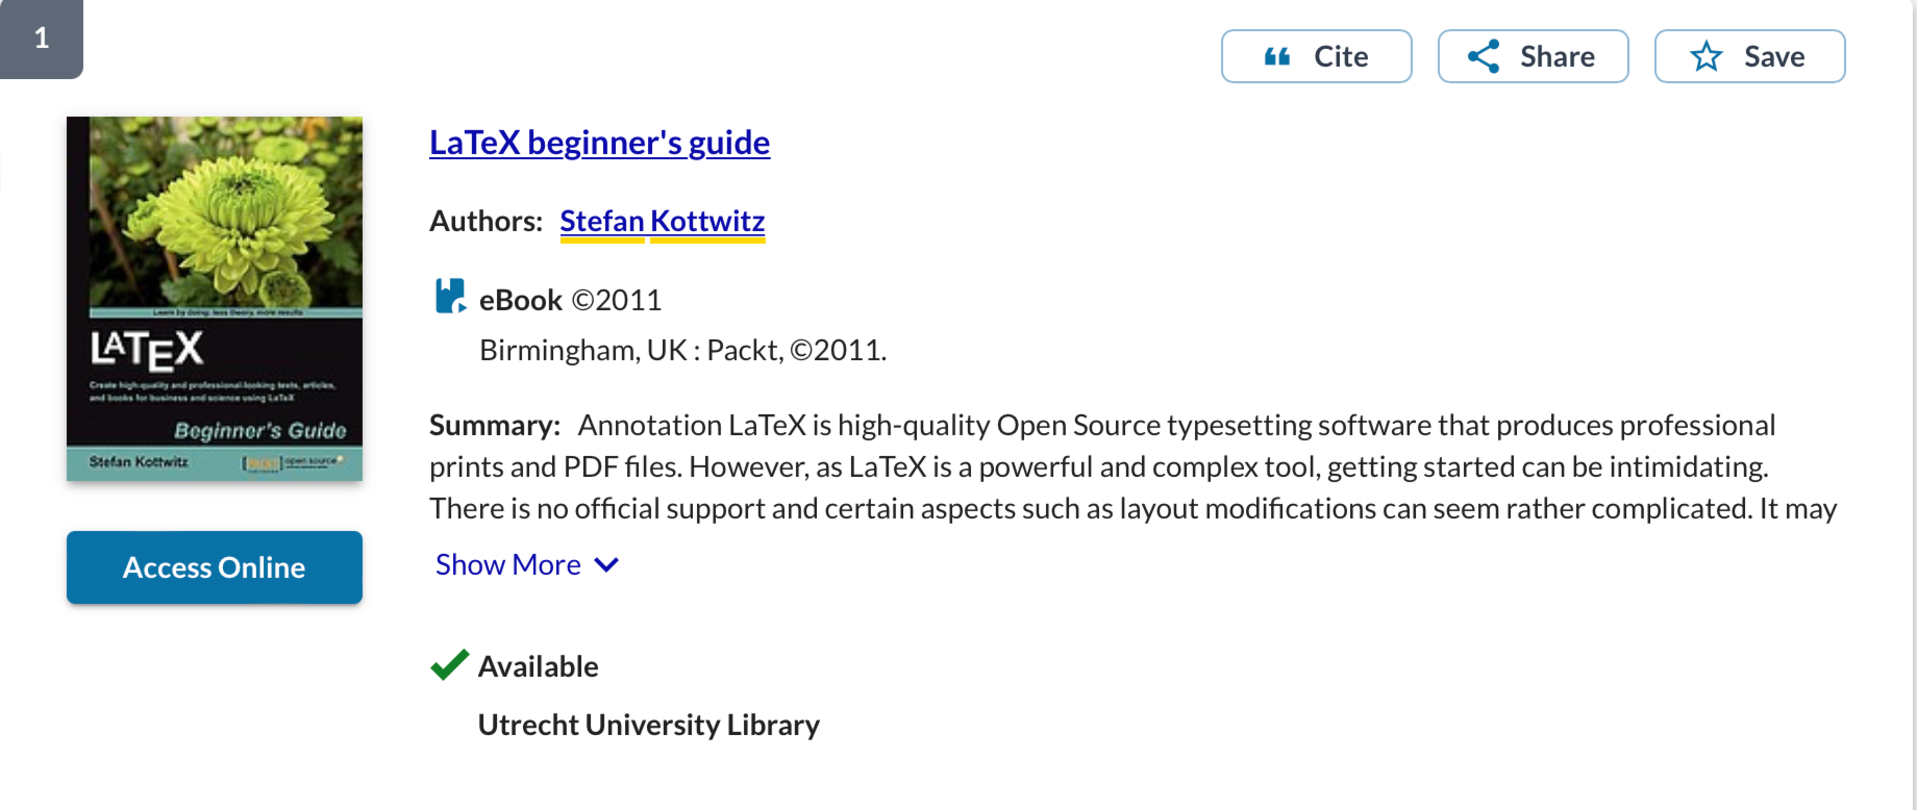
\includegraphics[width=0.8\textwidth]{images/kottwitz_book.pdf}
\end{figure}
\end{frame}
% \begin{frame}{Closing remarks}
The \TeX niCie organises a \textbf{thesis writing workshop} in februari 2023 and various other \LaTeX-workshops throughout the year.
These will be announced on our website at
\begin{center}
\fbox{\parbox[c][4cm][c]{8cm}{\centering \LARGE\url{a-eskwadraat.nl/LaTeX}}}
\end{center}
\end{frame}
\end{document}